\documentclass[]{article}
\usepackage{lmodern}
\usepackage{amssymb,amsmath}
\usepackage{ifxetex,ifluatex}
\usepackage{fixltx2e} % provides \textsubscript
\ifnum 0\ifxetex 1\fi\ifluatex 1\fi=0 % if pdftex
  \usepackage[T1]{fontenc}
  \usepackage[utf8]{inputenc}
\else % if luatex or xelatex
  \ifxetex
    \usepackage{mathspec}
  \else
    \usepackage{fontspec}
  \fi
  \defaultfontfeatures{Ligatures=TeX,Scale=MatchLowercase}
\fi
% use upquote if available, for straight quotes in verbatim environments
\IfFileExists{upquote.sty}{\usepackage{upquote}}{}
% use microtype if available
\IfFileExists{microtype.sty}{%
\usepackage{microtype}
\UseMicrotypeSet[protrusion]{basicmath} % disable protrusion for tt fonts
}{}
\usepackage[margin=1in]{geometry}
\usepackage{hyperref}
\hypersetup{unicode=true,
            pdftitle={Power Analysis Sample},
            pdfauthor={Dave Bridges},
            pdfborder={0 0 0},
            breaklinks=true}
\urlstyle{same}  % don't use monospace font for urls
\usepackage{graphicx,grffile}
\makeatletter
\def\maxwidth{\ifdim\Gin@nat@width>\linewidth\linewidth\else\Gin@nat@width\fi}
\def\maxheight{\ifdim\Gin@nat@height>\textheight\textheight\else\Gin@nat@height\fi}
\makeatother
% Scale images if necessary, so that they will not overflow the page
% margins by default, and it is still possible to overwrite the defaults
% using explicit options in \includegraphics[width, height, ...]{}
\setkeys{Gin}{width=\maxwidth,height=\maxheight,keepaspectratio}
\IfFileExists{parskip.sty}{%
\usepackage{parskip}
}{% else
\setlength{\parindent}{0pt}
\setlength{\parskip}{6pt plus 2pt minus 1pt}
}
\setlength{\emergencystretch}{3em}  % prevent overfull lines
\providecommand{\tightlist}{%
  \setlength{\itemsep}{0pt}\setlength{\parskip}{0pt}}
\setcounter{secnumdepth}{5}
% Redefines (sub)paragraphs to behave more like sections
\ifx\paragraph\undefined\else
\let\oldparagraph\paragraph
\renewcommand{\paragraph}[1]{\oldparagraph{#1}\mbox{}}
\fi
\ifx\subparagraph\undefined\else
\let\oldsubparagraph\subparagraph
\renewcommand{\subparagraph}[1]{\oldsubparagraph{#1}\mbox{}}
\fi

%%% Use protect on footnotes to avoid problems with footnotes in titles
\let\rmarkdownfootnote\footnote%
\def\footnote{\protect\rmarkdownfootnote}

%%% Change title format to be more compact
\usepackage{titling}

% Create subtitle command for use in maketitle
\newcommand{\subtitle}[1]{
  \posttitle{
    \begin{center}\large#1\end{center}
    }
}

\setlength{\droptitle}{-2em}
  \title{Power Analysis Sample}
  \pretitle{\vspace{\droptitle}\centering\huge}
  \posttitle{\par}
  \author{Dave Bridges}
  \preauthor{\centering\large\emph}
  \postauthor{\par}
  \predate{\centering\large\emph}
  \postdate{\par}
  \date{February 18, 2018}


\begin{document}
\maketitle

{
\setcounter{tocdepth}{2}
\tableofcontents
}
These data can be found in
/Users/davebrid/Documents/GitHub/Lab-Documents/Experimental
Policies/Power Analysis and this script was most recently run on Sun Feb
18 14:57:40 2018.

\section{Power Analysis}\label{power-analysis}

The assumptions set in this analysis are:

\begin{itemize}
\tightlist
\item
  The desired effect size is 5. This is what we want to power our
  analysis to be able to detect.
\item
  The standard deviation of the measurement is 3, in the same units as
  the effect size.
\item
  Therefore Cohen's \emph{d} is 1.667 or the number of standard
  deviations we want to be able to detect.
\item
  The acceptable false positive rate is 0.05. This is the percent chance
  that we observe something that is not actually true.
\item
  The acceptable false negative rate is 0.2. This is the percent chance
  that we miss something that is actually true.
\item
  The power of our analysis is set at 0.8.
\end{itemize}

\subsection{Calculate Number of
Animals}\label{calculate-number-of-animals}

At a standard power of 0.8 with a false positive rate of 0.05 and a
desired effect size of a 5 difference in percent fat mass we would need
\textbf{5.283} animals in each group.

\subsection{Calculate Effective Power}\label{calculate-effective-power}

The plot below shows how likely we are to detect a difference (the
power) as we vary the number of animals (x-axis) and the desired effect
size.

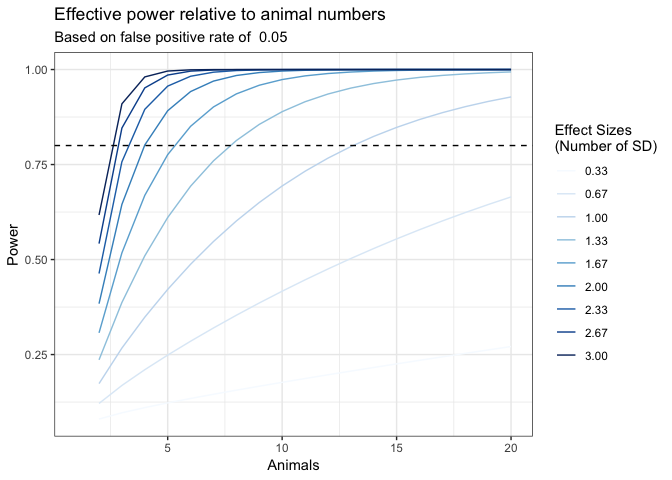
\includegraphics{figures/effect-size-plot-1.png}

\section{Session Information}\label{session-information}

\begin{verbatim}
## R version 3.4.2 (2017-09-28)
## Platform: x86_64-apple-darwin15.6.0 (64-bit)
## Running under: macOS High Sierra 10.13.3
## 
## Matrix products: default
## BLAS: /Library/Frameworks/R.framework/Versions/3.4/Resources/lib/libRblas.0.dylib
## LAPACK: /Library/Frameworks/R.framework/Versions/3.4/Resources/lib/libRlapack.dylib
## 
## locale:
## [1] en_US.UTF-8/en_US.UTF-8/en_US.UTF-8/C/en_US.UTF-8/en_US.UTF-8
## 
## attached base packages:
## [1] stats     graphics  grDevices utils     datasets  methods   base     
## 
## other attached packages:
## [1] RColorBrewer_1.1-2 pwr_1.2-1          ggplot2_2.2.1     
## [4] dplyr_0.7.4        tidyr_0.7.2        knitr_1.17        
## 
## loaded via a namespace (and not attached):
##  [1] Rcpp_0.12.14     bindr_0.1        magrittr_1.5     munsell_0.4.3   
##  [5] colorspace_1.3-2 R6_2.2.2         rlang_0.1.4      plyr_1.8.4      
##  [9] stringr_1.2.0    tools_3.4.2      grid_3.4.2       gtable_0.2.0    
## [13] htmltools_0.3.6  lazyeval_0.2.1   yaml_2.1.15      rprojroot_1.2   
## [17] digest_0.6.12    assertthat_0.2.0 tibble_1.3.4     bindrcpp_0.2    
## [21] purrr_0.2.4      glue_1.2.0       evaluate_0.10.1  rmarkdown_1.8   
## [25] labeling_0.3     stringi_1.1.6    compiler_3.4.2   scales_0.5.0    
## [29] backports_1.1.1  pkgconfig_2.0.1
\end{verbatim}


\end{document}
